\documentclass{beamer}

\usepackage{tikz}
\usepackage{subcaption}
\usepackage{amsmath,amssymb,amsthm}
\usetikzlibrary{arrows.meta,chains,%
	decorations.pathreplacing}

\usepackage{agda}
\usepackage{catchfilebetweentags}

\usepackage{bbm}
\usepackage[greek,english]{babel}
\usepackage{alphabeta}

\usepackage{ucs}
\usepackage[utf8]{inputenc}
\usepackage{autofe}

\usepackage{newunicodechar}
\newunicodechar{ₑ}{\textsubscript{e}}
\newunicodechar{∀}{\ensuremath{\mathnormal\forall}}
\newunicodechar{ℕ}{$\mathbb{N}$}
\newunicodechar{𝕓}{$\mathbbm{b}$}
\newunicodechar{⊢}{$\vdash$}
\newunicodechar{∶}{:}
\newunicodechar{∷}{::}
\newunicodechar{₀}{$_0$}
\newunicodechar{₁}{$_1$}
\newunicodechar{₂}{$_2$}
\newunicodechar{₃}{$_3$}
\newunicodechar{↔}{$\leftrightarrow$}
\newunicodechar{ᶠ}{\textsuperscript{f}}
\newunicodechar{ᵇ}{\textsuperscript{b}}
\newunicodechar{↝}{$\leadsto$}
\newunicodechar{ᵃ}{\textsuperscript{a}}
\newunicodechar{ˣ}{\textsuperscript{x}}
\newunicodechar{≡}{$\equiv$}


\begin{document}
\frame{
	\frametitle{Reversibly erasing the first of a pair}
	\begin{center}
		\scalebox{0.6}{
		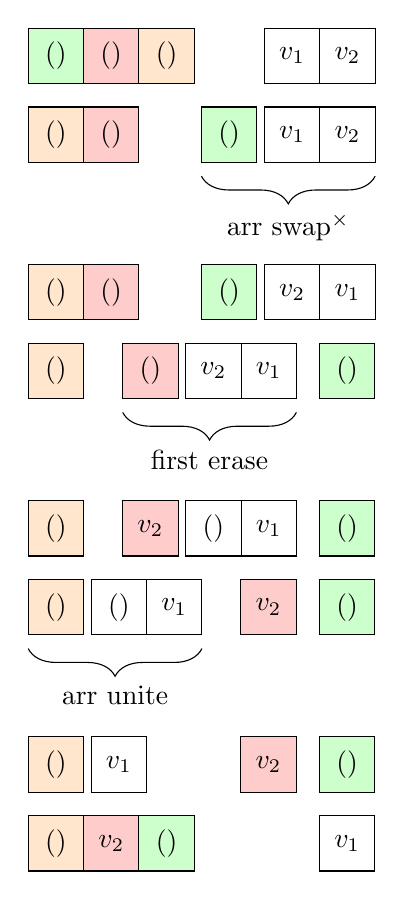
\begin{tikzpicture}[
			%  -{Stealth[length = 2.5pt]},
			start chain =1 going right,
			start chain =2 going right,
			start chain =3 going right,
			start chain =4 going right,
			start chain =5 going right,
			start chain =6 going right,
			start chain =7 going right,
			start chain =8 going right,
			start chain =9 going right,
			start chain =10 going right,
			node distance = 0pt,
			MyStyle/.style={draw, minimum width=2em, minimum height=2em, 
				outer sep=0pt, on chain=1},
			C/.style={draw, minimum width=2em, minimum height=2em, 
				outer sep=0pt, on chain=3},
			C1/.style={draw, minimum width=2em, minimum height=2em, 
				outer sep=0pt, on chain=2},
			C2/.style={draw, minimum width=2em, minimum height=2em, 
				outer sep=0pt, on chain=4},
			C3/.style={draw, minimum width=2em, minimum height=2em, 
				outer sep=0pt, on chain=5},
			C4/.style={draw, minimum width=2em, minimum height=2em, 
				outer sep=0pt, on chain=6},
			C5/.style={draw, minimum width=2em, minimum height=2em, 
				outer sep=0pt, on chain=7},
			C6/.style={draw, minimum width=2em, minimum height=2em, 
				outer sep=0pt, on chain=8},
			C7/.style={draw, minimum width=2em, minimum height=2em, 
				outer sep=0pt, on chain=9},
			C8/.style={draw, minimum width=2em, minimum height=2em, 
				outer sep=0pt, on chain=10},
			%thick,scale=0.75, every node/.style={scale=0.75}
			]
			\node [MyStyle, fill=green, fill opacity =0.2, text opacity = 1] (1) at (0,0) {$()$};
			\node [MyStyle, fill=red, fill opacity =0.2, text opacity = 1] (2) {$()$};
			\node [MyStyle, fill=orange, fill opacity =0.2, text opacity = 1] (3) {$()$};
			
			\node [C] (8) at (3,0) {$v_1$};
			\node [C] (9) {$v_2$};
			
			
			%\draw[decorate,decoration={brace, amplitude=10pt, raise=5pt, mirror}]
			%(1.south west) to node[black,midway,below= 15pt] {heap} (3.south east);%
			
			\node [C1, fill=orange, fill opacity =0.2, text opacity = 1] (a) at (0,-1) {$()$};
			\node [C1, fill=red, fill opacity =0.2, text opacity = 1] (b) {$()$};
			\node [draw, minimum width=2em, minimum height=2em, 
			outer sep=0pt, fill=green, fill opacity =0.2, text opacity = 1] (c) at (2.2,-1) {$()$};
			
			\node [C2] (d) at (3,-1) {$v_1$};
			\node [C2] (e) {$v_2$};
			
			
			\draw[decorate,decoration={brace, amplitude=10pt, raise=5pt, mirror}]
			(c.south west) to node[black,midway,below= 15pt] {arr swap$^\times$} (e.south east);%
			
			
			%\draw[decorate,decoration={brace, amplitude=10pt, raise=5pt, mirror}]
			% (a.south west) to node[black,midway,below= 15pt] {$k$-elements} (c.south east);%
			
			\node [C4, fill=orange, fill opacity =0.2, text opacity = 1] (a) at (0,-3) {$()$};
			\node [C4, fill=red, fill opacity =0.2, text opacity = 1] (b) {$()$};
			\node [draw, minimum width=2em, minimum height=2em, 
			outer sep=0pt, fill=green, fill opacity =0.2, text opacity = 1] (c1) at (2.2,-3) {$()$};
			
			\node [C3] (d1) at (3,-3) {$v_2$};
			\node [C3] (e1) {$v_1$};
			
			\node [draw, minimum width=2em, minimum height=2em, 
			outer sep=0pt, fill=orange, fill opacity =0.2, text opacity = 1] (a) at (0,-4) {$()$};
			\node [draw, minimum width=2em, minimum height=2em, 
			outer sep=0pt, fill=red, fill opacity =0.2, text opacity = 1] (b) at (1.2,-4) {$()$};
			
			\node [C5] (d1) at (2,-4) {$v_2$};
			\node [C5] (e1) {$v_1$};
			\node [draw, minimum width=2em, minimum height=2em, 
			outer sep=0pt, fill=green, fill opacity =0.2, text opacity = 1] (c1) at (3.7,-4) {$()$};
			
			\draw[decorate,decoration={brace, amplitude=10pt, raise=5pt, mirror}]
			(b.south west) to node[black,midway,below= 15pt] {first erase} (e1.south east);%
			
			\node [draw, minimum width=2em, minimum height=2em, 
			outer sep=0pt, fill=orange, fill opacity =0.2, text opacity = 1] (a) at (0,-6) {$()$};
			\node [draw, minimum width=2em, minimum height=2em, 
			outer sep=0pt, fill=red, fill opacity =0.2, text opacity = 1] (b) at (1.2,-6) {$v_2$};
			
			\node [C6] (d1) at (2,-6) {$()$};
			\node [C6] (e1) {$v_1$};
			\node [draw, minimum width=2em, minimum height=2em, 
			outer sep=0pt, fill=green, fill opacity =0.2, text opacity = 1] (c1) at (3.7,-6) {$()$};
			
			
			\node [draw, minimum width=2em, minimum height=2em, 
			outer sep=0pt, fill=orange, fill opacity =0.2, text opacity = 1] (a) at (0,-7) {$()$};
			\node [C7] (d1) at (0.8,-7) {$()$};
			\node [C7] (e1) {$v_1$};
			
			\node [draw, minimum width=2em, minimum height=2em, 
			outer sep=0pt, fill=green, fill opacity =0.2, text opacity = 1] (c1) at (3.7,-7) {$()$};
			
			\node [draw, minimum width=2em, minimum height=2em, 
			outer sep=0pt, fill=red, fill opacity =0.2, text opacity = 1] (b) at (2.7,-7) {$v_2$};
			\draw[decorate,decoration={brace, amplitude=10pt, raise=5pt, mirror}]
			(a.south west) to node[black,midway,below= 15pt] {arr unite} (e1.south east);%
			
			\node [draw, minimum width=2em, minimum height=2em, 
			outer sep=0pt, fill=orange, fill opacity =0.2, text opacity = 1] (a) at (0,-9) {$()$};
			\node [draw, minimum width=2em, minimum height=2em, 
			outer sep=0pt] (d1) at (0.8,-9) {$v_1$};
			
			\node [draw, minimum width=2em, minimum height=2em, 
			outer sep=0pt, fill=green, fill opacity =0.2, text opacity = 1] (c1) at (3.7,-9) {$()$};
			
			\node [draw, minimum width=2em, minimum height=2em, 
			outer sep=0pt, fill=red, fill opacity =0.2, text opacity = 1] (b) at (2.7,-9) {$v_2$};
			
			\node [C8, fill=orange, fill opacity =0.2, text opacity = 1] (1) at (0,-10) {$()$};
			\node [C8, fill=red, fill opacity =0.2, text opacity = 1] (2) {$v_2$};
			\node [C8, fill=green, fill opacity =0.2, text opacity = 1] (3) {$()$};
			
			\node [draw, minimum width=2em, minimum height=2em, 
			outer sep=0pt] (c1) at (3.7,-10) {$v_1$}; 
		\end{tikzpicture}
	}
	\end{center}
	
}	

\frame
{ 
	\frametitle{Implementation Overview}
	
	\begin{center}
		\begin{figure}[!htbp]
			\begin{subfigure}{0.5\textwidth}
				\centering
				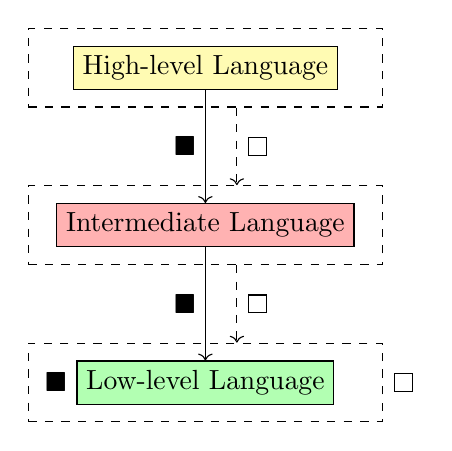
\begin{tikzpicture}[node distance = 2cm,auto]
					
					% high-level box
					\node[draw=black,dashed,minimum width=4.5cm,minimum height = 1cm,font=\Large] (main1){};
					\node[draw,fill=yellow!30](main11) at (main1.center){High-level Language};
					
					%mid-level
					\node[draw=black,dashed,minimum width=4.5cm,minimum height = 1cm,font=\Large] (main2) [below of=main1]{};
					\node[draw,fill=red!30](main21) at (main2.center){Intermediate Language};
					
					%low-level
					\node[draw=black,dashed,minimum width=4.5cm,minimum height = 1cm,label=right:$\qedsymbol$] (main3) [below of=main2]{};
					\node[draw,fill=green!30,label=left:$\blacksquare$](main31) at (main3.center){Low-level Language};
					
					\draw [->,dashed] ([xshift=0.4 cm]main1.south) -- ([xshift=0.4 cm]main2.north) node[midway, right] {$\qedsymbol$};
					\draw [->,dashed] ([xshift=0.4 cm]main2.south) -- ([xshift=0.4 cm]main3.north)  node[midway, right] {$\qedsymbol$};
					
					\draw [->] (main11) -- (main21) node[midway, left] {$\blacksquare$};
					\draw[->] (main21) -- (main31) node[midway, left] {$\blacksquare$};
					
				\end{tikzpicture}
				
			\end{subfigure}
			\hfill
			\begin{subfigure}{0.45\textwidth}
				\textbf{--} Completed Implementation
				
				
				- - TODO: Implementation 
				
				
				$\blacksquare$ Completed Proof
				
				
				$\qedsymbol$ TODO: Proof 
			\end{subfigure}
		\end{figure}
	\end{center}
} 

\frame{
	\frametitle{Language definitions}
	Evaluation in high-level language LET:
	
	\ExecuteMetaData[Languages/Let.tex]{eval-declare}
		
    Evaluation in low-level language $\Pi$:
	
	\ExecuteMetaData[Languages/PiTyped.tex]{pi-eval}
	
	Evaluation in intermediate language ML$_{\Pi}$:
	\ExecuteMetaData[Languages/MLPi.tex]{mlpi-eval}
}

\frame{
	\frametitle{Translations and proofs}
	Proof of $\Pi$'s reversibility:
	
	\ExecuteMetaData[Languages/PiTyped.tex]{pi-rev}
	
	T$_1$ that translates programs from LET to ML$_\Pi$ is correct:
	\ExecuteMetaData[../../Translations/latex/Translations/T1.tex]{T1-proof}
	
		T$_2$ that translates programs from ML$_\Pi$ to $\Pi$ is correct:
	\ExecuteMetaData[../../Translations/latex/Translations/T2.tex]{T2-proof}
}



\end{document}